\documentclass[tikz]{standalone}

\usepackage{settings}
\usetikzlibrary{graphs.standard}
\usegdlibrary{trees,force,circular}

\begin{document}
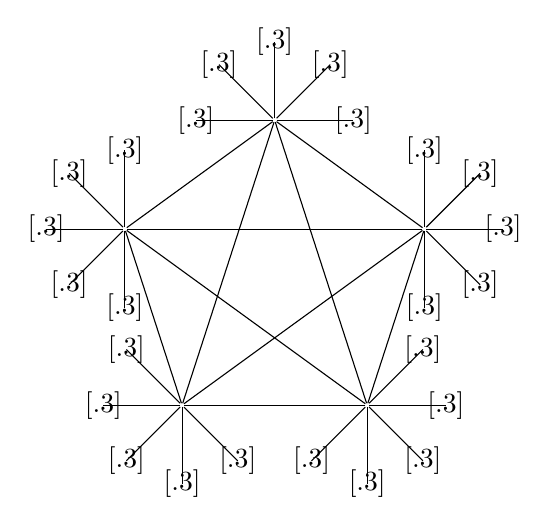
\begin{tikzpicture} [inner sep=0pt]
  \graph { subgraph K_n [n=5, name=R, clockwise, radius=2cm, nodes={as={\router}}] };

  \foreach \i/\a in {1/-45, 2/-135, 3/180, 4/90, 5/45} {
    \foreach \j in {1,...,5}{
      \draw (R \i) -- +(\j*45+\a:1cm) node {\router[.3]};
    }
  }
\end{tikzpicture}
\end{document}
%%% Local Variables:
%%% mode: latex
%%% TeX-master: t
%%% End:
